\subsection{Region Two Construction (Special Considerations)}

The R2 chambers, which were designed and constructed by Old Dominion University 
in collaboration with Jefferson Laboratory, are the middle of the three  
drift-chamber packages.  They track all charged particles in the magnetic field 
of the torus near the point of maximum sagitta.  The six identical R2 sectors 
are approximately equilateral triangular boxes with 3~m sides. 
They are located at a radius of $\approx$3~m from the nominal target location.  
  
The R2 chambers were designed with ultra-thin endplates that were thin enough
to be wholly within the ``shadow'' cast by the torus cryostat; in other words,
any track that does not strike the torus cryostat will enter the active fiducial 
volume of the R2 chambers. 
All chamber support hardware and electronics had to fit 
entirely within this shadow region.

Fig.~\ref{dc-corner} shows a slice through a chamber endplate (R2 in this case)
showing some of the wire positioning hardware and attachment of the electronics 
boards.

%%%%%%%%%%%%%%%%%%%%%% Figure : DC Sector Schematic %%%%%%%%%%%%%%%%%%%%%%
\begin{figure}[htpb]   
\vspace{8cm}
\special{psfile=img/r2_inserts.eps hscale=70 vscale=70 hoffset=80 voffset=30}  
\caption{\small{Schematic cross-sectional view of the R2 endplate showing
wire-positioning hardware.}}
\label{dc-corner}
\end{figure}   
%%%%%%%%%%%%%%%%%%%%%%%%%%%%%%%%%%%%%%%%%%%%%%%%%%%%%%%%%%%%%

The R2 chambers have to operate 
in a magnetic field up to 2~T, and the chambers have to withstand any rapid 
changes in magnetic field, such as what might occur due to a magnet quench.
The R2 endplates are constructed from 2-cm thick Stesalit 4411W, a disordered 
epoxy-fiberglass composite commonly used in wire-chamber construction
\cite{stesalit}, and known not to cause aging problems~\cite{stesalitaging}.  
Using a nonconducting material eliminates any possible forces on the endplate 
due to eddy currents produced during a magnetic-field quench.  

The ``Stesalit'' composite is not very stiff and, if not reinforced, would
bend excessively under the load of wire tension.  So, as in the case of
the R1 chambers, the R2 endplates were a composite structure with
stainless steel stifferners.  Fig.~\ref{dcr2-endplate} shows an assembly drawing of an R2 endplate.

%%%%%%%%%%%%%%%%%%%%%% Figure : generic chamber sketch %%%%%%%%%%%%%%%%%%%%%%
\begin{figure}[hbpt]   
\vspace{4.7cm}
\begin{picture}(35,35)
\put(30,-25)
{\hbox{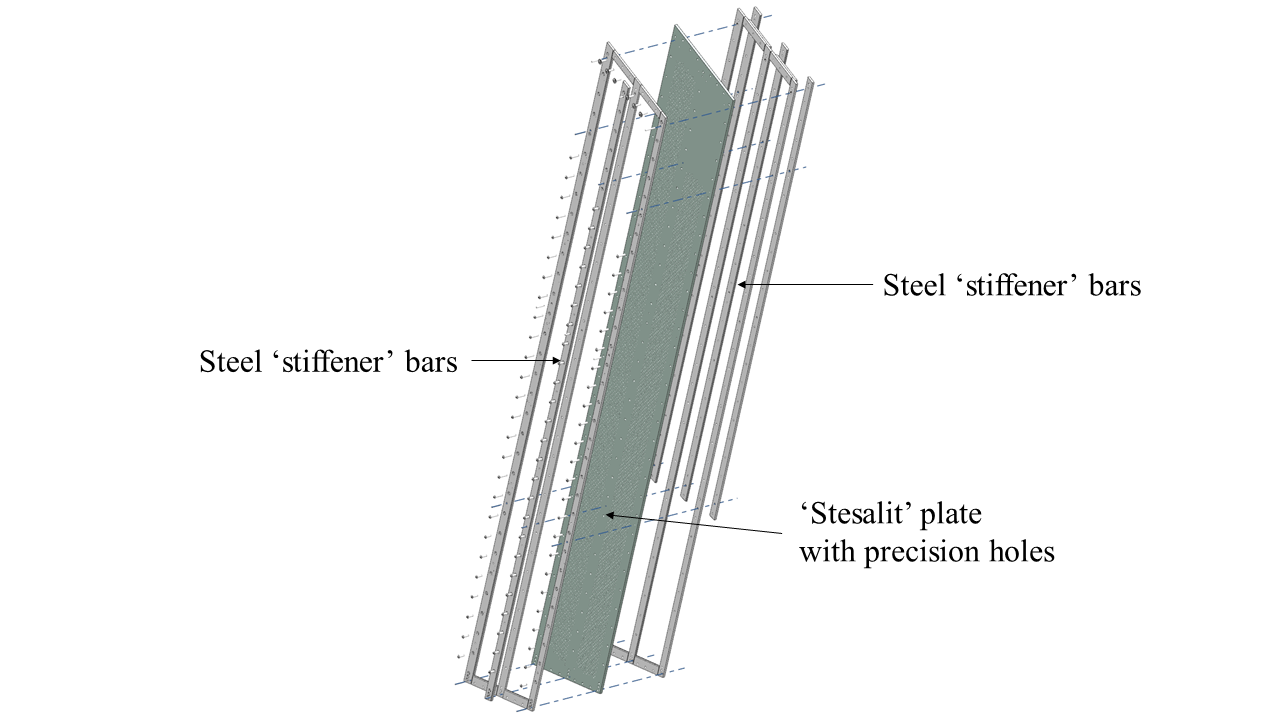
\includegraphics[width=0.6\columnwidth,natwidth=610,natheight=642]{img/dcr2-endplate.png}}}
\end{picture}
\caption{\small{A R2 endplate assembly with its components highlighted.}}
\label{dcr2-endplate}
\end{figure}   
%%%%%%%%%%%%%%%%%%%%%%%%%%%%%%%%%%%%%%%%%%%%%%%%%%%%%%%%%%%%%%

The use of a non-conducting endplate also allows the trumpets that position the wires to be 
essentially flush with the endplates, 
rather than having to insulate the trumpets from the conducting endplates as in 
the other two Regions (see Fig.~\ref{dc-corner}).  This reduced the thickness of 
the inactive region by 1 to 2~cm.




 
